\section{FlexGraph Architecture}

In this section, we describes the overall architecture of the FlexGraph Accelerator.

\subsection{FlexGraph Computing Model}

\begin{figure}[htbp]
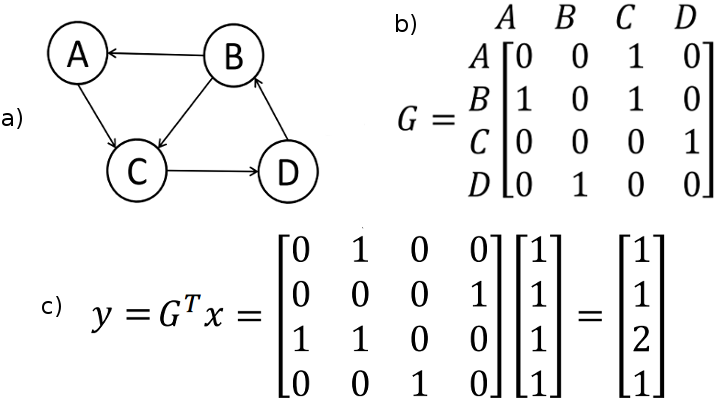
\includegraphics[width=0.4\textwidth]{figures/graph_vertex_programming}
\caption{Graph Vertex Programming}
\label{fig:graph_vertex_programming}
\end{figure}

FlexGraph's architecture is based on GraphMat \cite{GraphMat}'s vertex computing paradigm where a graph algorithm is described as a linear algebra set of operations operating on sparse matrix with input vertices. Figure \ref{fig:graph_vertex_programming} shows an example where graph (a) is converted into matrix (b), allowing us to execute operations on the graph using simple matrix vertex multiplication (c). This above example will to generate the number of incoming edges for each vertex. All GraphMat algorithms, Breadth First Search (BFS) \cite{BFS}, PageRank \cite{PageRank}, Single Source Shortest-Path (SSSP) \cite{SSSP}, etc.. are expressed in this fashion such that computation can be efficiently accelerated in hardware. In FlexGraph, we accelerate the matrix vertex computation on the FPGA, instead of executing it on the multi-core host processor.

\subsection{The Doubly Compressed Sparse Matrix}

\begin{figure}[htbp]
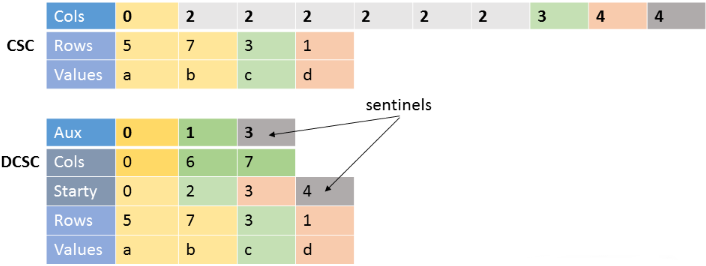
\includegraphics[width=0.4\textwidth]{figures/DCSC_matrix_format}
\caption{DCSC hyperspace matrix format}
\label{fig:DCSC_matrix_format}
\end{figure}

Most Data Analytics graphs are represented in a sparse matrix format to save memory space due to the large amount of empty edges that exist. FlexGraph's matrices are stored using a Doubly Compressed Sparse Column (DCSC) \cite{DCSC} format. The format allows minimal traversal into the sparse matrix structure, saving necessary memory bandwidth when fetching empty columns. Figure \ref{fig:DCSC_matrix_format} shows a sample matrix A = \{(0,5,a), (0,7,b), (6,3,c), (7,1,d)\} with four non-zero edges (src, dst, weight) encoded using DCSC versus the conventional CSC \cite{CSC} format. It is encoded as follows: The CSC encoding for this matrix is as follows: The \textit{Cols} buffer holds the column ranges stored as incremental distances from first value, which allows efficient packing of consecutive non-zero columns. The limitation of this scheme is that it entries are replicated to skip empty columns. \textit{Rows} and \textit{Values} hold the corresponding rows and values referenced by a given non-empty column.
The traversal over CSC requires accessing all consecutive column ranges \textit{(cols[i+2] - cols[i])} even though most of the distances are empty. DCSC saves on bandwidth by using an additional indirection  buffer inside its structure to only encode non-zero columns. It is important to note that the saving this format introduced additional space and compute overhead that only pays off when the matrix is very large and sparse, a prevalent characteristic of Graph Analytics datasets.

\subsection{Sparse Matrix Multiplication Kernel}

\begin{lstlisting}[language=Python, caption=Pseudocode for SPMV kernel]
def SPMV_kernel(x_values, x_activemask) :
  y_values = {0}, y_activemask = {0}
    for col in cols :                        # +	
      (a_x, rows) = coldata[col]             # *
      x_value  = x_values[a_x]               # *
      x_active = x_activemask[a_x]           # *
      if (x_active):                         # ?
        for row in rows:                     # +
          (a_y, a_value) = rowdata[row]      # *
          y_values[a_y] += a_value * x_value # *
          x_activemask[a_y] = true           # *
  return (y_values, y_activemask)
\end{lstlisting}

\subsection{FlexGraph Micro-architecture}

\section{FlexGraph Parallelization}

\subsection{DCSC Matrix partitioning}

\subsection{Precessing Tasks Scheduling}

\subsection{Synchronising Memory Writes for Dirty Masks}

\section{FlexGraph Optimizations}

\subsection{Optimizing Memory Accesses via Stream Buffers}

\subsection{Caching Vertex Values and Masks}